% Please use the skeleton file you have received in the 
% invitation-to-submit email, where your data are already
% filled in. Otherwise please make sure you insert your 
% data according to the instructions in PoSauthmanual.pdf
\documentclass{PoS}

\usepackage[utf8]{inputenc}
\usepackage{acronym}
\usepackage{alltt}
\usepackage[usenames,dvipsnames]{xcolor}

\acrodef{ARC}{Advanced Resource Connector}
\acrodef{xRSL}{Extended Resource Specification Language}

\title{Computational workflows with GC3Pe}

\ShortTitle{Computational workflows with GC3Pie}

\author{\speaker{Sergio MAFFIOLETTI}\\
        GC3: Grid Computing Competence Center\\
        University of Zurich \\
         E-mail: \email{sergio.maffioletti@gc3.uzh.ch}}

\author{Riccardo Murri\\
        GC3: Grid Computing Competence Center\\
        University of Zurich \\
        E-mail: \email{riccardo.murri@gmail.com}}

\author{Tyanko Aleksiev\\
        GC3: Grid Computing Competence Center\\
        University of Zurich \\
        E-mail: \email{tyanko.aleksiev@gmail.com}}



\abstract{
  % Intro va rifatta probabilmente.
  This paper present GC3Pie \cite{gc3pie}, a python library to ease the
  development of scalable and robust High Throughput data analysis
  tools. Most of the current distributed computing middlewares as well
  as most of the in-house grown scripts fall short in reaching the
  scaling and reliability factors required by the ever growing demand
  of large data analysis. GC3Pie provides mechanisms to automitise the
  execution and the monitoring of large collection of applications
  while, at the same time, provides simple data structures and
  interfaces to steer the behaviour of the underlying system in an
  application-centric perspective. The goal of GC3Pie is to embody the
  common execution and monitorig processing part of large data
  analysis while moving most decision making logic to the application
  level; like, for example, the reaction to certain types of failures,
  the validation of the application execution or the brokering of the
  computing resources driven by application fidelity metrics.
  This allows to write application specific tools that take full
  control of the underlying computing and data infrastructure, as
  opposite to current middleware stacks that are trying to embody the
  full control of the execution logic thus reducing the flexibility of
  the entire system as they prevent applications to define their own
  expected behaviour of the system.}

\FullConference{EGI Community Forum 2012 / EMI Second Technical Conference\\
          26-30 March, 2012\\
           Munich, Germany}

\begin{document}

\section{What is GC3Pie ?}
GC3Pie is a library of Python classes to execute and control
applications on distributed computing resources (e.g., SGE clusters
and ARC-based grids).
 
GC3Pie is object-oriented: basic classes abstract the generic and
repetitive part of application scripting, and let you focus on coding
what is specific to your use case. Generic services provided by GC3Pie
include: asynchronous job execution, programmatic generation of
template files, checkpoint/restart workflow execution.

GC3Pie is a toolkit: it provides the building blocks to write Python
scripts to run large computational campaigns (e.g., to analyze a vast
dataset or explore a parameter space), and to combine several tasks
into a dynamic workflow.

\section{How is GC3Pie different ?}
Most execution engines represent workflows as data (e.g., some XML
format). GC3Pie lets you write Python code instead: you write your
workflow as a set of Python classes so the entire workflow logic is
expressed in a plain programming language. This means that it is easy
to create loops and conditionally branch execution, for example.
 
Unlike other Python frameworks for distributing computation, e.g.,
Celery \cite{celery} or Pyro \cite{pyro}, GC3Pie is designed to
coordinate the execution of independent Applications (often
pre-existing and written in another language): with GC3Pie you write
Python code to steer the computation, not to perform it. 

\section{Workflows with GC3Pie}
GC3Pie encourages a compositional approach for building workflows: the
unit of job composition is called a \texttt{Task} in GC3Libs. An
\texttt{Application} is the primary instance of a
\texttt{Task}. However, a single task can be composed of many
applications. A task is a composite object: tasks can be composed of
other tasks. Workflows are built by composing tasks in different
ways. A \emph{workflow} is a task, too.

The classes \texttt{SequentialTaskCollection} and
\texttt{ParallelTaskCollection} are the basic compositions of Tasks; by
subclassing them you define how to coordinate the execution of
Tasks. For example, retry the execution of a certain step in a
sequence, or stop a parallel parameter sweep when a certain percentage
of the tasks in it are successfully done. 
 
\texttt{TaskCollections} are mutable objects, so Python code can alter them on
the fly, while a composition is running. This allows the creation of
dynamic workflows, whose structure is not fixed in advance, rather
built in response to external events.

\section{A real-world example: (Economic) Model calibration using
  Global Optimization}

The presented workflow shows how a differential evolution optimizer is
implemented with the GC3Pie library to support the analysis of a
computationally intense economic model. The paper \cite{Jones2011}
seeks to understand the co-movement of interest rates and exchange
rates. The economic model is calibrated with data for five countries
with major currencies.
 
To illustrate the explanatory power of the model, the countries'
preference parameters are chosen to bring the simulated economies
close to the real world. The resulting 10-dimensional optimization
problem of a non-convex function is undertaken with the help of the
GC3Pie library. 

\texttt{GFPSequence} (see fig. \ref{fig1}), a
SequentialTaskCollection, implements the differential evolution
optimizer: each optimization iteration is one sequential task. When
initialized, the optimizer generates an initial population of size n
for the N-dimensional parameters (N=10).  

The whole population is evaluated in parallel as a
\texttt{ParallelTaskCollection}. Each of the n tasks within
the collection is an \texttt{Application} instance, a C++
implementation of the economic model that simulates the interaction of
two economies. 
 
After the \texttt{GFPParallel} has completed, the
\texttt{GFPSequence.next()} method checks for convergence, otherwise
generates  a new population of size n and evaluates it.


The \texttt{SessionBasedScript} class provides a command line interface and
allows running several optimizations in parallel.

\section{Wrokflow structure}
For each optimization, a workflow is started. A driver script class
\texttt{SessionBasedScript} provides support for running several Tasks
in parallel:

The SessionBasedScript class implements a command line interface to
manage a session consisting of the tasks so created.

\begin{center}
  \begin{minipage}{0.5\linewidth}
\begin{alltt}
class \textcolor{blue}{GFPScript}(\textcolor{Lavender}{SessionBasedScript}):
  def new_tasks(self):
    for ctry1, ctry2 in self.country_pairs:
      # add tasks to the session
      yield (jobname,# unique identifier 
             \textcolor{Purple}{GFPSequence}  # task class
             [ args ],  # creation arguments 
             { kwargs })# creation keywords
\end{alltt}
    \end{minipage}
  \end{center}

A succession of Tasks is implemented through a
\texttt{SequentialTaskCollection}. Tasks in the collection are
executed one after the other; after one of them completes, the
\texttt{next()} method is called to determine what step to take:
continue execution with another task, or stop. The \texttt{next()}
method can modify the collection, or re-run tasks already run. It is
thus possible to implement indefinite loops, that repeat until a
certain condition is met. 

\begin{center}
  \begin{minipage}{0.5\linewidth}
\begin{alltt}
class  \textcolor{Purple}{GFPSequence}(\textcolor{Lavender}{SequentialTaskCollection}):
  def __init__(self, ...):
    SequentialsTaskCollection.__init__(
      self, [ tasks ], ...)
  def next(self, done):
    if self.tasks[done].converged == True:
      return Run.State.TERMINATED
    else:
      # run another optimization step,
      # with altered parameters
      new_params = ...
      self.tasks.add( \textcolor{YellowGreen}{GFParallel}(new_params))
\end{alltt}
  \end{minipage}
\end{center}

Several simulations are run in parallel, one for each combination of
input parameters; input files for each simulations are created using a
template mechanism.
 
The \texttt{ParallelTaskCollection} class is used to manage concurrent
Tasks; subclass it to create specialized collections:
 
\begin{center}
  \begin{minipage}{0.5\linewidth}
\begin{alltt}
class \textcolor{YellowGreen}{GFPParallel}(\textcolor{Lavender}{ParallelTaskCollection}):
  def __init__(self, params..., **kwargs):
    # create Task collection from parameters
    tasks = [ \textcolor{BlueViolet}{GFPApplication}(...) ]
    ParallelTaskCollection.__init__(
      self, tasks, **kwargs)
\end{alltt}
    \end{minipage}
  \end{center}

\texttt{Applications} are the basic Tasks that comprise a workflow in
GC3Pie. An Application is just a UNIX process, i.e., any command that
can be run from the shell command line.  The Application class should
be subclassed to specify error-checking policies and post-processing
of output files:

\begin{center}
  \begin{minipage}{0.5\linewidth}
\begin{alltt}
class \textcolor{BlueViolet}{GFPApplication}(\textcolor{Lavender}{Application}):
def __init__(self, ...):
  Application.__init__(
      executable="./forwardPremiumOut",
      arguments=[ "1", "2", "3" ],
      inputs=[ "input.file.name" ],
      outputs=[ "out.file", "out.directory" ])

  def terminated(self):
    # this gets called once the Task is done
    if "simulation.out" in self.outputs:
      self.execution.returncode = 0 # success
    else:
      self.execution.returncode = 1 # fail!
\end{alltt}
  \end{minipage}
\end{center}

\begin{figure}
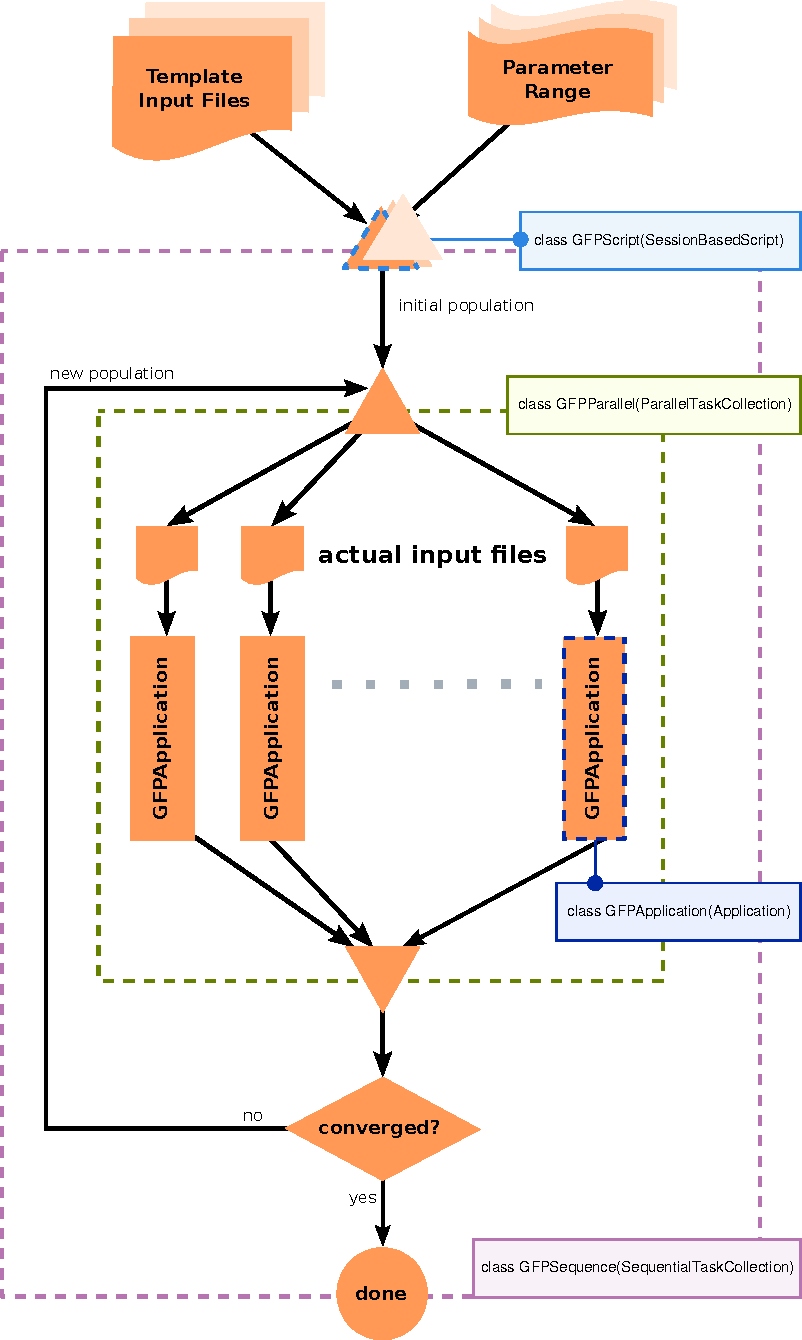
\includegraphics[width=.6\textwidth]{gc3pie_fig1.pdf}
\caption{The GFPremium workflow}
\label{fig1}
\end{figure}


The workflow has been integrated in a suite called \texttt{gpremium} that has
been used by a research group from the Department of Banking and
Finance a the University of Zurich
(http://www.bf.uzh.ch/). A
total of 796024062 jobs and an aggregated walltime of 221118 cpu/hours
has been generated through the \texttt{gpremium} suite.


\section{Conclusion}
This paper has presented how complex computational workflows could be
programmatically model using the GC3Pie framework. Instead of
expressing the workflow logic using a defined workflow description
language as in many data-driven systems, GC3Pie allows to use simple
and yet effective data structures to programmatically compose tasks.
GC3Pie is an open source project under GPL license available at at
http://code.google.com/p/gc3pie/.


\begin{thebibliography}{99}
  \bibitem{Jones2011} Jonen B., Scheuring S. Time-Varying International
    Diversification and the Forward Premium (working paper). Institut
    für Banking und Finance, University of Zurich, 2011.
  \bibitem{Prince2005} Price K.V., Storn R.M., Lampinen J.A. Differential
    evolution: a practical approach to global optimization. Springer,
    2005.
  \bibitem{pyro} Pyro: http://packages.python.org/Pyro4/
  \bibitem{celery} Celery: Distributed Task Queue
    http://celeryproject.org/
  \bibitem{gc3pie} GC3Pie. http://code.google.com/p/gc3pie/
  \bibitem{gpremium} Gpremium, is a GC3Pie application available
    throught the GC3Pie repository. http://code.google.com/p/gc3pie/
\end{thebibliography}

\end{document}



